%!TEX root = main.tex

\subsection{\textbf{RQ1:} Ho do software developers manage merge conflicts?}\label{RQ1}

\boldif{Results from interviews indicated that a common model of operating with merge conflicts exists.}
To understand how developers manage merge conflicts, we asked interview participants to describe their current processes for handling merge conflict.

\boldif{\textit{Add anecdotal quotes and descriptions from interviews to highlight these observations.}}
Participants talked about different steps that they follow, including using tools that alert them to potential or current merge conflicts, processes for analyzing and understanding conflicting code prior to implementing a resolution, and the use of tools for validating that their resolution worked.
As an example, P3 said:
\begin{quoting}
\textit{``Part of my job on the integration team requires that I check for bad regressions. I use scripts to track patches as they're being backported, so I know when and where to look if [a patch] introduces a conflict. [\ldots] And once I've fixed [the conflict], I try to compare with the previous version to make sure [the code] works in a similar way.''}
\end{quoting}

\boldif{Provide descriptions that link the stages of Merge Conflict model to this quote. Use it to drive description of simplified model description paragraph}

\boldif{Based on these anecdotal observations, we construct an initial model of the processes that developers employ when working with merge conflicts, see Fig.~\ref{model}.}
Our interview and survey results suggest that developers follow a series of phases through which they manage the life-cycle of individual merge conflicts.
We construct a model of the developer processes for managing merge conflicts and examine each phase in detail.
Figure~\ref{model} provides an illustration of this model. 
It consists of four phases: \emph{awareness, planning, resolution,} and \emph{evaluation.}

\boldif{Discuss the fact that no other studies have shown that a model exists for merge conflicts}

\begin{figure}[!htbp]
\centering
\fbox{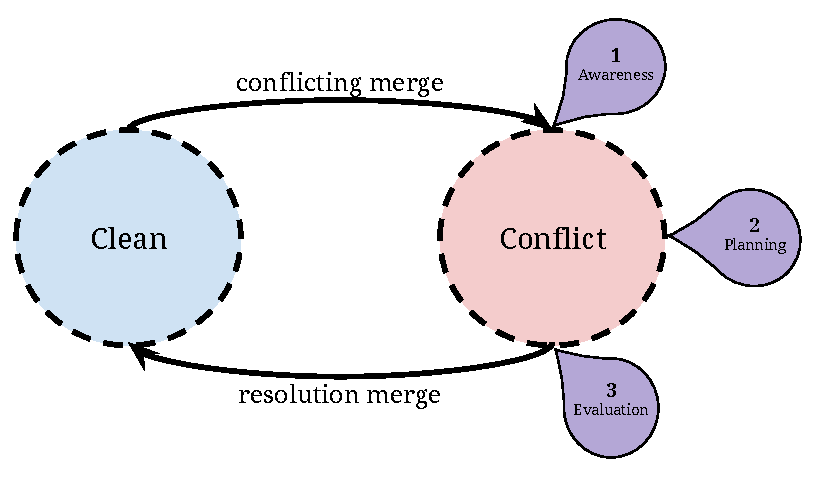
\includegraphics[width=0.90\textwidth,keepaspectratio]{imgs/MergeConflictModel}}
\caption{Model of Developer Processes for Managing Merge Conflicts. Developers alternate between \textit{clean} and \textit{conflicting} states of code. Beginning from (1)~\textit{development}, developers maintain (2)~\textit{awareness} of conflicts within the codebase in different ways. Once aware, developers begin (3)~\textit{planning} for a (4)~\textit{resolution} to fix the conflict. And finally, developers (5)~\textit{evaluate} the effectiveness of their deployed resolutions (returning to \emph{planning} if the resolution failed).\vspace*{-0.3\baselineskip}}
\label{model}
\end{figure}

\boldif{Awareness is how developers become aware}
First, the \emph{awareness} phase consists of the actions developers take to become aware of merge conflicts.
This could be passive, as the developer will become aware of a merge conflict when attempting to merge changes or perform a pull.
At the other end of the spectrum are developers who \emph{proactively} monitor for merge conflicts as they write code.
They are actively looking for changes that might be problematic, either manually or through the use of specialized tools.

\boldif{Planning is when developers plan their future actions}
Second, the \emph{planning} phase occurs after the developer has become aware that a conflict has occurred, and they are about to tackle the conflict.
This includes the decision of when they will try and resolve the conflict.
Some developers might try and resolve it immediately, while others might postpone the resolution.
Some might change their strategy depending on the conflict, incoming deadlines, or availability of resources.
This also includes other actions, such as if they are going to tackle the conflict alone, or collaborate with other developers knowledgeable in the area of conflict~\cite{CostaSarma}.

\boldif{Resolution is the action of implementing a resolution. Mundane and well understood, so we focus on the other three.}
Third, the \emph{resolution} phase represents the implementation of the planned resolution.
Several tools exist that help in this phase~\cite{nishimura,mens2002state,Brun2011}.
Here we focus on the difficulties that developers face during these resolution implementations (see Section~\ref{RQ2}).

\boldif{Evaluation is how developers check that their solution is correct}
Finally, after the conflict has been resolved, developers enter in the \emph{evaluation} phase.
In this phase, the developer has to evaluate their resolution before considering the conflict as resolved.
This is to ensure the correctness of the resulting code.
Possible actions during this stage includes compiling the source code.
Developers wanting more guarantees can go a step further and run the tests.
Finally, some groups have policies such as code reviews that need to be performed on the merge conflict resolution.
 
\boldif{To explore and validate this model, we asked developers to reflect upon how they become aware of merge conflicts, how they plan for merge conflict resolutions, and how they evaluate their resolutions in the \textit{Processes Survey}~(S1).}
In order to explore and validate this model, and our assumptions, we conducted the \emph{Processes Survey}~(S1).
Our aim in this survey was to understand how developers become aware of merge conflicts (what steps they take, what tools they use, etc.).
Also, we wanted to investigate their strategies for dealing with merge conflicts and how they decide whether the resolution has addressed all of their concerns.

\boldif{We present the results to these research questions in Sections~\ref{RQ1a}, \ref{RQ1b}, and \ref{RQ1c}.}
Sections~\ref{RQ1a}, \ref{RQ1b}, and \ref{RQ1c} presents the results to these research questions.

\subsubsection{\textbf{RQ1a:} How do software developers become \textbf{aware} of merge conflicts?}\label{RQ1a}

\boldif{Developers use 2 methods for becoming aware of merge conflicts: proactive and reactive.}
From the \textit{Processes Survey}~(S1) we found that 29.41\% of participants do not actively monitor for merge conflicts during their development activities.
For the rest of the developers who answered with \emph{yes} or \emph{sometimes} (61.77\%), we identified 61 different tools mentioned in 126 instances.

\nsubsection{Reactive and Proactive Monitoring for Merge Conflicts}

\boldif{Reactive detection only notifies developers that a merge conflict \emph{has happened}. Developers use it to minimize the size/complexity of the conflict, or it's impact on the team.}
Reactive monitoring for merge conflicts notifies the developer that a conflict has already occurred.
However, developers still use this process to manage or reduce the complexity of a conflict.
For the developers who answered that they monitor for merge conflicts (replied either \emph{yes} or \emph{sometimes}), we found that 73.68\% (42 out of 57 responses; 6 participants left this field blank) described reactive processes.
For example, participant S1--48 said they use integration tools to detect merge problems before they advance to testing:
\begin{quotation}
	[\ldots] integration tests tell us if builds are breaking and we use those to locate merge conflicts. [\ldots] we use it to catch merge bugs before they go to smoke testing for release
\end{quotation}
And participant S1--64 mentioned that they try to solve merge conflicts early in order to minimize disruptions to the team:
\begin{quotation}
	We try to catch conflicts early so that fewer developers have to be involved in looking at broken code.
\end{quotation}

\boldif{Proactive monitoring allows devs to detect MC before they happen. However, it is more involved, as it requires a lot more manual effort from the developers.}
Proactive monitoring allows developers to preemptively catch merge conflicts before they happen.
15 participants (14.71\%) mentioned they achieved this by manually tracking incoming changes, such as participant S1--35 who indicated:
\begin{quotation}
	I monitor commit logs before I begin merging branches so that I see any potentially overlapping code that will break the merge.
\end{quotation}
Other teams rely more on communication.
This can happen during regular team meetings, to make sure that everybody is aware of each other's tasks, for example participant S1--46 said:
\begin{quotation}
	[\ldots] standups allow us to know where everyone is working that week.
\end{quotation}
While 10 participants (9.80\%) indicated that they broadcast their changes in order to notify team members if they will make breaking changes.
For example, participant S1--102 indicated that team members:
\begin{quotation}
	[\ldots] send emails before making breaking changes to the API or related sub-modules.
\end{quotation}

\boldif{Developers do not regularly actively monitor for merge conflicts. ...}
To conclude, only a third of developers actively monitor for merge conflicts.
When developers are caught unaware of the conflict, they are more likely to be interrupted by it.
This can lead to more frustration, as they do not have any warning of when the conflict will occur and whether they have the time to deal with it immediately.

\nsubsection{Tools for Monitoring for Merge Conflicts}

\boldif{The tools that developers use allow for only a \emph{reactive} approach.}
Examining the tools used by participants with reactive processes, we find that 87.72\% of these participants rely on version control systems (e.g. Git, SVN, TFS, CVS), while 21.05\% use continuous integration systems (e.g. Jenkins, Travis CI, TeamCity).
Table~\ref{s1_toolset} presents the top 10 tools developers use when monitoring for merge conflicts, including the totals for both reactive and proactive strategies.

Additionally, we examine the tools used by participants with proactive processes.
We find that all participants with a proactive strategy rely on version control systems, and 33.33\% use continuous integration systems.
Additionally, 26.66\% of proactive participants use code analysis tools (e.g. SonarQube, Code Climate).

We find that the majority of tools used by developers for merge conflict monitoring are built to only support reactive strategies, and that multiple tools must be used in conjunction for a proactive approach.

%\boldif{Devs do not use existing workspace awareness tools that come from the acadmemia.}
%When collaborating, developers generally rely on passive communication tools, like email, to coordinate.
%Developers are currently not leveraging the functionalities provided by many research prototypes (e.g., Palant\'{i}r~\cite{palantir}, Crystal~\cite{Brun2011}) that are specifically designed to facilitate proactive conflict detection.

\begin{table}[!htbp]
\renewcommand{\arraystretch}{1.3}
\caption{Merge Awareness Toolsets (Top 10) from Processes Survey (S1)}
\label{s1_toolset}
\centering
\begin{tabularx}{\textwidth}{ll|cc|c}
\toprule
% \textbf{Par.}\parnote{Par. = Total number of survey participants using each tool.}
% \vspace*{-0.3\baselineskip}
  \parnoteclear % tabularx will otherwise add each note thrice
  Tool\parnote{\textit{Processes Survey}~(S1) participants were allowed to provide multiple tools. 57 out of 102 participants (56\%) indicated the use of at least one merge awareness tool.} & Description & Proactive\parnote{Participants using this tool with a proactive strategy.} & Reactive\parnote{Participants using this tool with reactive strategy.} & Total\parnote{Total number of survey participants using each particular tool.}\\
\midrule
  Git & Version Control System & 10 & 30 & 40\\
  Email (unspecified) & Email Client or System & 2 & 4 & 6\\
  GitHub & Project Hosting Site & 2 & 5 & 7\\
  SVN & Version Control System & 0 & 4 & 4\\
  Visual Studio & IDE & 1 & 2 & 3\\
  PagerDuty & IT Incident Manag. Sys. & 0 & 3 & 3\\
  GitLab & Project Hosting Site & 2 & 1 & 3\\
  Jenkins & Continuous Integration & 0 & 3 & 3\\
  VCS (unspecified) & Version Control System & 2 & 2 & 4\\
  Team Foundation Server & Version Control System & 1 & 1 & 2\\
\bottomrule
\end{tabularx}
\parnotes
\end{table}


\boldif{Therefore their approaches are mostly \emph{reactive,} and their tool selection reflects that.}
To summarize, we find that developers employ \emph{reactive} processes, even if they are proactive in monitoring for merge conflicts once they have occurred.
This can be seen as a consequence of the tools that developers have at their disposal.
All the tools mentioned support only a \emph{reactive} approach, which biases developers towards one particular solution.
If developers want a more \emph{proactive} approach, then based on the tools they use, they need to come up with their own solution.
The most often cited techniques involve increasing communication among developers.
While this technique might be effective in small teams, it scales very poorly and cannot be effectively used in larger organizations~\cite{brooks1974mythical}.

\boldif{All the above point towards a need for better collaborative tools, that promote a proactive approach}
Finally, our results point to the conclusion that developers are not aware of existing proactive tools (e.g. Palant\'{i}r~\cite{sarma_palantir:_2003}, Crystal~\cite{Brun2011}), and are therefore not leveraging those tools to actively monitor for merge conflicts.
However, developers are trying to mitigate the severity of merge conflicts by attempting to resolve them as soon as they become aware.

\subsubsection{\textbf{RQ1b:} How do software developers \textbf{plan} for merge conflict resolutions?}\label{RQ1b}

\boldif{Developers use different strategies for dealing with MC}
When encountering a merge conflict, developers follow different strategies.
They can either: (a) defer the merge conflict to a later date, or; (b) solve the conflict.
In the \textit{Processes Survey}~(S1) we sought an understanding of these strategies and when developers use them.
The tools that developers use when implementing merge conflict resolutions are discussed in Section~\ref{RQ3}.

\nsubsection{Deferring Responses to Merge Conflicts}

\boldif{25\% of developers consider all conflicts as being equally urgent.}
One quarter of our participants consider all merge conflicts to be equally urgent.
This means that they will always solve the conflict as soon as the 
We can assume that most developers will interrupt their work regardless of the type of merge conflict.
Therefore, they will give the same level of attention, for example, to a conflict generated by whitespace or formatting changes, as a conflict that is generated by overlapping logical changes. 
%TODO: Make sure this fits in the flow.

\boldif{The first option is that they might defer the MC, for a later time}
The easiest option when encountering a merge conflict is to simply not deal with it.
Indeed, we found that 56.18\% of participants have deferred at least once when responding to a merge conflict.
The reasons for deferring are varied and listed in Table~\ref{s1_deferring_response}.

The location and complexity of conflicting code (D1, D2) were the most selected factors, and match the top difficulty factors of merge conflicts (F1, F2) as described in Section~\ref{difficulty-factors}.
% TODO Add a conclusion statement about the meaning of these factors being top in both tables.

As the third most selected factor, \textit{ownership of the conflicting code}~(D3) indicates that the deferral is not always temporal, but can also be logistical when developers defer to other team members.
Participant S1--8 succinctly defines the role ownership impacts his workflow as:
\begin{quotation}
	Code is mine? I fix it. Code is others? I submit PR or bug reports.
\end{quotation}
We additionally asked participants to rate the degree to which code ownership factors into their overall merge conflict strategy, and participants indicate that code ownership factors \textit{about half the time} in their strategy of code ownership (mean: $3.21$ on a 5-point Likert-type scale).
Only 10.11\% of participants indicated that code ownership \textit{never} factors into their resolution strategy.

\begin{table}[!htbp]
\renewcommand{\arraystretch}{1.2}
\caption{Factors in Deferring Responses to Merge Conflicts from Processes Survey (S1)}
\label{s1_deferring_response}
\centering
\begin{tabularx}{\textwidth}{>{\rowmac}c | >{\rowmac}l | >{\rowmac}c | >{\rowmac}r <{\clearrow}}
\toprule
  \parnoteclear % tabularx will otherwise add each note thrice
  Factor & Description & \# Selections\parnote{\textit{Processes Survey}~(S1) participants were allowed to select multiple factors. 44 out of 102 participants (43\%) selected more than one factor.\vspace*{-0.9\baselineskip}} & Percentage (\%)\textsuperscript{i} \\
\midrule
  D1 & Complexity of the conflicting code & 36 & 25.00\% \\
  D2 & Number of conflicting code locations & 32 & 22.22\% \\
  D3 & Ownership of the conflicting code & 25 & 17.36\% \\
  D4 & Size of the conflicting code & 20 & 13.89\% \\
  D5 & Approaching deadlines & 13 & 9.03\% \\
  D6 & Work schedule constraints & 2 & 1.39\% \\
  D7 & Other\hspace{4.6cm} & 7 & 4.86\% \\
\bottomrule
\end{tabularx}
\parnotes
\end{table}

\boldif{60\% of developers defer a merge conflict, at least once. However, there doesn't seem to be a systematic understanding of the effect of such a deferral.}
%Our study results indicate that 60\% of developers have deferred a merge conflict at least once. 
While developers have listed multiple reasons for deferral, two stand out: complexity and the number of conflicting locations.
Both of these reasons indicate that a developer is more likely to defer if the conflict resolution appears to be lengthy, either because the potential changes are non-trivial or because there are many smaller conflicts requiring the developers' attention.

\nsubsection{Deferring Response to Merge Conflicts}

\boldif{Deferring can have bad consequences, including increased complexity and delaying features. Organizations have sometimes changed the policy to prevent this.}
Deferring the merge conflict resolution comes with a price.
Table~\ref{effects-deferral} shows the top effects of deferring a response to a merge conflict.
The most common effect was that developers have had to stop the development (\emph{Stop the Presses,} 15 responses) in order to resolve the conflicts.
This halt in development includes asking team members to also refrain from adding any additional code into the codebase.
The second most common effect is the \textit{increased complexity} of the conflicts (E2), reported by nine participants.
Participant S1--93 noted that:
\begin{quotation}
	Deferring a merge conflict simply kicks the can down the road (or off a cliff). Typically resolving the conflict only gets more difficult as time passes.
\end{quotation}
Participant S1--70 even hinted that the increased complexity can be quite severe, on an order of magnitude greater than if the conflict were addressed immediately:
\begin{quotation}
	Untangling takes days instead of minutes when it gets too out of hand.
\end{quotation}
In some cases, features had to be removed from releases, in order for integration problems to be mitigated and the conflict to be successfully resolved. S1--5 said:
\begin{quotation}
	We have had several releases come up short in new features because they got delayed by integration problems.
\end{quotation}
Finally, in order to prevent similar problems arising, some organizations have instituted \textit{policy changes} (E4) to prevent this from happening in the future. Participant S1--46 said:
\begin{quotation}
	We've had devs push a bunch of code up before going on holiday and mucking up a release, so we've instituted an all hands on deck policy for the 2 weeks leading up to a major release
\end{quotation}

\boldif{However, some effect can be severe, including impact to customers, or having to reimplement features.}
In one extreme case, participant S1--9 reported that an unresolved merge conflict affected production software (E7), which resulted in downtime of the product, as it broke functionality:
\begin{quotation}
	Broke the app for customers until we could get a patch pushed [\ldots].
\end{quotation}
Finally, the merge conflicts can get too severe and intractable for developers to cope with the complexities.
In these types of situations, developers have to resort to the \emph{Nuclear Option} (E5), where they scrap their changes and manually reimplement them.
Such as in the case of S1--102, who said:
\begin{quotation}
	Uh.... KABOOM! More changes came in and everything piled up. Nothing to do but wipe it all back to clean and start trying to piece things back together.
\end{quotation}

\begin{table}[!htbp]
\renewcommand{\arraystretch}{1.2}
\caption{Effects of Deferring Response to a Merge Conflict from Processes Survey (S1)}
\label{effects-deferral}
\centering
\begin{tabularx}{\textwidth}{>{\rowmac}c | >{\rowmac}l | >{\rowmac}c | >{\rowmac}r <{\clearrow}}
\toprule
  \parnoteclear % tabularx will otherwise add each note thrice
  Effect & Description & \# Participants\parnote{46 out of 102 participants (45.1\%) provided a description of the effects of deferring.\vspace*{-0.8\baselineskip}} & Percentage (\%)\textsuperscript{i} \\
\midrule
  E1 & Stop the Presses & 15 & 32.61\% \\
  E2 & Increased complexity & 9 & 19.57\% \\
  E3 & Non-operation effects & 5 & 10.87\% \\
  E4 & Policy/cultural changes & 3 & 6.52\% \\
  E5 & The Nuclear Option & 2 & 4.35\% \\
  E6 & Physical manifestations & 1 & 2.17\% \\
  E7 & Impact beyond the organization \hspace{1cm} & 2 & 2.17\% \\
\bottomrule
\end{tabularx}
\parnotes
\end{table}
\vspace{0.8em}

\boldif{The results of such a deferral can be disastrous. However, it is difficult to make an assessment of the effect of the deferral when the decision to defer is being made.} 
The results of deferring can be disastrous. 
%Participants reported having to throw away code (the \emph{Nuclear Option}) and even rising to the level of customers and users experiencing broken functionality and loss of access.
However, it is difficult to assess a deferral to determine if it will turn a single merge conflict into a larger problem.
Tools could provide such information; responding to developers with enough information to make accurate and informed decisions in order to prevent further issues down the line.

\nsubsection{Attempting Resolution \& Initial Strategies}

\boldif{If they have not deferred, they need to understand the (changes in the) conflict}
When developers don't defer their response, they have to resolve the conflicts now.
They primarily approach merge conflicts by \textit{examining the merge} (U1), \textit{analyzing or manipulating the code} (U2), or \textit{examining the code} (U3).
Table~\ref{s1_understanding_code} lists all six strategies described by the \textit{Processes Survey}~(S1) participants.

\begin{table}[!htbp]
\renewcommand{\arraystretch}{1.2}
\caption{Initial Strategies for Understanding Conflicting Code from Processes Survey (S1)}
\label{s1_understanding_code}
\centering
\begin{tabularx}{\textwidth}{>{\rowmac}c | >{\rowmac}l | >{\rowmac}c | >{\rowmac}r <{\clearrow}}
\toprule
  \parnoteclear % tabularx will otherwise add each note thrice
  Strategy & Description & \# Participants\parnote{79 out of 102 participants (77\%) provided a description of their initial strategy.\vspace*{-0.3\baselineskip}} & Percentage (\%)\textsuperscript{i} \\
\midrule
  U1 & Examining the merge & 26 & 32.91\% \\
  U2 & Analysis/manipulation of the code & 19 & 24.05\% \\
  U3 & Examining the code & 18 & 22.79\% \\
  U4 & Focus on design concerns & 8 & 10.13\% \\
  U5 & Examine project organization & 6 & 7.60\% \\
  U6 & No strategy\hspace{3.5cm} & 2 & 2.53\% \\
\bottomrule
\end{tabularx}
\parnotes
\end{table}
\vspace{0.8em}

\boldif{The most common strategies for understanding the conflict are examining the conflict and analysis/manipulation of the code.}
Participant S1--44 described their strategy of \textit{examining the merge}~(U1) as:
\begin{quotation}
	Reviewing the most recent commits (comments and code) to see whether it's a shallow conflict or not.
\end{quotation}
	And participant S1--69 indicated their strategy of analyzing the code (U2) involves:
\begin{quotation}
[\ldots] determining if the merge conflict involves important functionality; stepping through with a debugger helps.
\end{quotation}
Overall, we find that developers initially focus on the code involved in the merge conflict or information related to the merge itself.

\boldif{Surprisingly, some developers do not have a strategy for MCR}
Surprisingly, we found that two of our participants (2.53\% of participants) indicated that they \textit{``don't have a strategy''} or \textit{``mostly try to fix it as soon as possible.''}

%\begin{figure}[!htbp]
%\centering
%\fbox{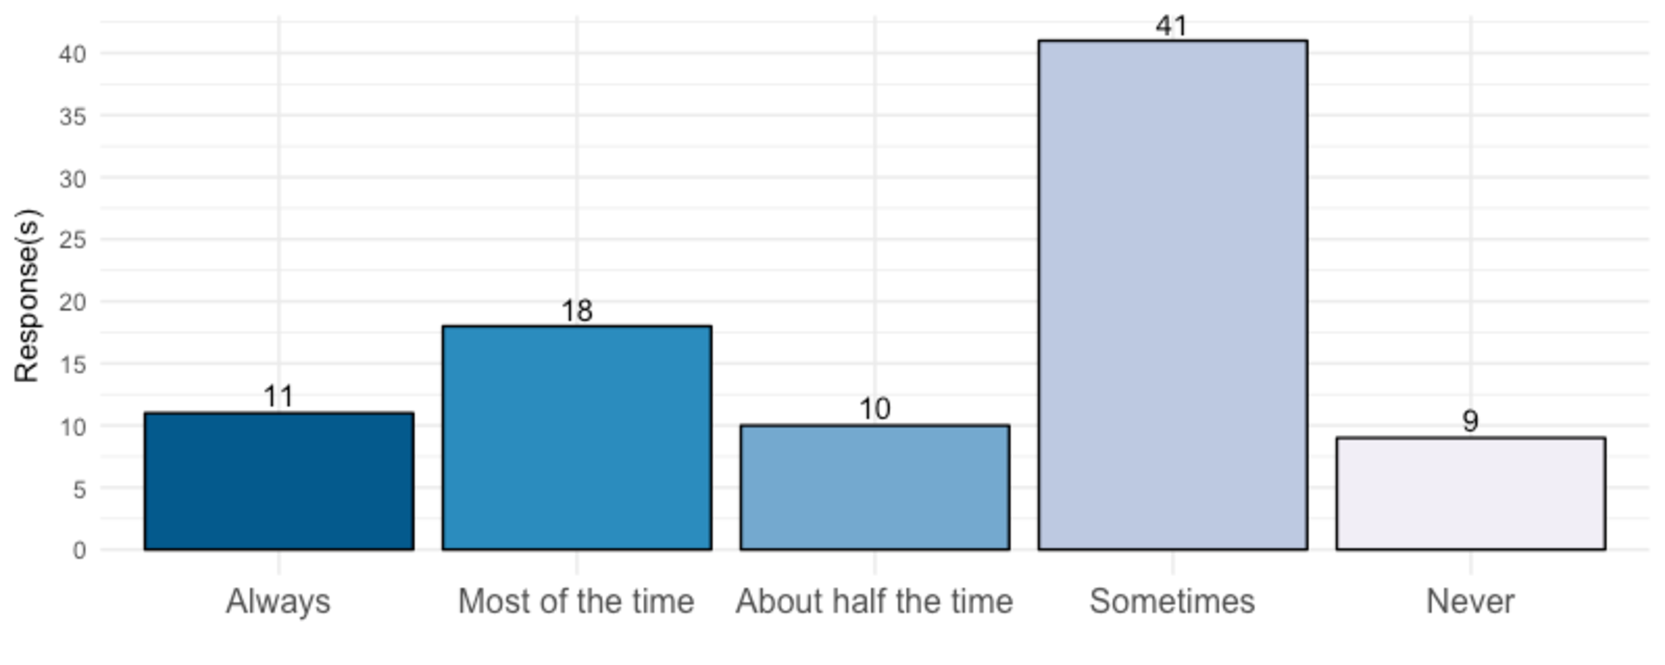
\includegraphics[width=0.98\textwidth,keepaspectratio]{imgs/CodeOwnershipFactor}}
%\caption{Degree of Code Ownership as a Factor in Merge Conflict Strategies. Scale: 1 is \textit{Always} and 5 is \textit{Never}. 89 out of 102 participants (87.26\%) provided a response to this question in the \textit{Processes Survey}~(S1).\vspace*{-0.3\baselineskip}}
%\label{fig:code-ownership-resolution}
%\end{figure}

To conclude, developers reported that expertise in the area of the conflicting code is one of the top factors in determining the difficulty of a merge conflict.
Additionally, developers also indicate that increases in perceived complexity of merge conflicts is strongly linked with the degree of difficulty in resolving them.
Therefore, developers' perceptions and intuition are relied on throughout the implementation of their resolution.

\subsubsection{\textbf{RQ1c}: How do software developers \textbf{evaluate} merge conflict resolutions?}\label{RQ1c}

After implementing a merge conflict resolution, software developers must evaluate whether their resolution has returned the codebase to a clean state.
We asked developers to select the conditions (from interviews) that they use to determine whether their resolution has successfully addressed the merge conflict.

\nsubsection{Success Conditions for Merge Conflict Resolutions}

In the \textit{Exploratory Interviews}, developers described six common conditions they considered important in their evaluation.
We asked \textit{Processes Survey}~(S1) participants to select from this list of conditions, including an \textit{Other} option to elicit additional conditions.
Only two developers selected that condition, indicating ``performance tests showing similar performance'' and ``client approval.''
We received 324 selections from 89 participants and present the aggregated results in Table~\ref{conditionsSuccess}.

\begin{table}[!htbp]
\caption{Conditions of Successful Merge Conflict Resolutions from Processes Survey (S1)\textsuperscript{i}}
\label{conditionsSuccess}
\centering
\begin{tabularx}{\textwidth}{@{}lr|*{7}{C}c@{}}
\toprule
	&
	& C1
	& C2
	& C3
	& C4
	& C5
	& C6
	& C7 \\
\midrule
	C1 & All tests pass & \textbf{67} & & & & & & \\
	C2 & Code compiles & 50 & \textbf{67} & & & & & \\
	C3 & Code looks correct & 50 & 54 & \textbf{66} & & & & \\
	C4 & VCS warmings gone & 38 & 42 & 41 & 51 & & & \\
	C5 & Code reviewed & 32 & 31 & 27 & 25 & 38 & & \\
	C6 & Merged to production & 27 & 27 & 27 & 26 & 19 & 33 & \\
	C7 & Other & 2 & 2 & 0 & 0 & 0 & 0 & 2 \\
\bottomrule
    \multicolumn{9}{c}{\noindent\parbox[t]{11.7cm}{\vspace{0.4em}\textsuperscript{i}\hspace{0.2em}\textit{Processes Survey}~(S1) participants were allowed to select multiple conditions. Each entry represents the number of participants that selected both of the conditions indicated for the column and row. 68 out of 102 participants (67\%) selected three or more conditions.}\vspace*{-0.3\baselineskip}} \\
\end{tabularx}
\end{table}

\textit{All tests pass} (C1), \textit{code successfully compiles} (C2), and \textit{code looks correct (i.e. visual test passes)} (C3) were the most commonly selected conditions required for a successful merge resolution.
These results are in line with existing literature showing that testing (C1) can be used for validating program functionality and correctness~\cite{beizer1984software,tian2005software}. %and have been fundamental to development processes such as test-driven development for several years~\cite{beck2003test}.
Similarly, the use of compilers to validate code (C2) as being executable and in good-working order will be familiar to any developer using a compiled programming language.

The use of visual inspection as a measure of successful merge conflict resolutions is surprising to us, given that \textit{complexity of conflicting lines of code}~(F1) is the highest rate factor for impact on merge conflict difficulty~\cite{mckee2017software}.
Inspecting code requires time and expertise in the area of conflicting code.
However, the survey participants that selected \textit{code looks correct (i.e. visual test passes)}~(C3) had a mean of 9.2 years of programming experience, which is only slightly higher than the overall mean of 9.0 years of programming experience.

Looking at the combination of \textit{code looks correct (i.e. visual test passes)}~(C3) with the other conditions, we find that 54 participants also selected \textit{all tests pass}~(C1) (52.9\%).
As the most common co-occuring selections, we conclude that although developers rely upon their expertise to visually inspect a merge conflict resolution, they also run the test suite to validate their evaluation.
Experience can play a big factor, as this method (C3) is highly subjective.

\boldif{Tests are still the most common criteria for determining a merge conflict resolution successful.}
The two most common evaluation criteria that developers mentioned are that the \emph{code compiles,} and that \emph{all tests pass.}
However, less then half selected both options.
While tests passing can be considered a good criteria of a successful resolution, the fact that the code compiles is not.
Even if the code compiles, there can be logical errors that are introduced during the merge resolution process, especially if the resolution was difficult.

\boldif{Only a minority of developers mention that code review is part of their success criteria}
Interestingly, only a minority of developers (37.25\%) mentioned code reviews as part of their success criteria.
%TODO add citation for the code review part
While code reviews are an effective way to detect bugs introduced by changes in the codebase, the practice appears to have not been adopted for code changed during merge conflict resolutions.

\nsubsection{Merge Resolution Evaluation Toolsets}

From the \textit{Exploratory Interviews}, we identified five categories of software development tools that developers mention in relation to merge conflicts.
In the \textit{Processes Survey}~(S1), we asked the developers to identify the tools they use when evaluating a merge conflict resolution.
We received 204 selections from 89 participants.
The aggregated results are presented in Table~\ref{resolution-evaluation-tools}, ranked according to the percentage of participants that selected each toolset.

\begin{table}[!htbp]
\renewcommand{\arraystretch}{1.2}
\caption{Merge Resolution Evaluation Toolsets from Processes Survey (S1)}
\label{resolution-evaluation-tools}
\centering
\begin{tabularx}{\textwidth}{>{\rowmac}l | >{\rowmac}c | >{\rowmac}r <{\clearrow}}
\toprule
  \parnoteclear % tabularx will otherwise add each note thrice
  Description & \# Selections\parnote{\textit{Processes Survey}~(S1) participants were allowed to select multiple toolsets. 64 out of 89 participants (71.91\%) selected multiple toolsets.\vspace*{-0.3\baselineskip}} & Percentage (\%)\textsuperscript{i} \\
\midrule
  Version Control Systems (e.g. Git, Subversion, CVS) & 82 & 92.14\% \\
  Continuous Integration (e.g. TravisCI, Jenkins, TFS) & 62 & 69.66\% \\
  Program Analysis Tools (e.g. Coverity, CodeSonar) & 26 & 29.21\% \\
  DevOps Tools (e.g. Nagios, Monit, Kabana) & 17 & 19.10\% \\
  Release Management Tools (e.g. Chef, Puppet, Salt) & 9 & 10.11\% \\
  Other Tools & 8 & 8.99\% \\
\bottomrule
\end{tabularx}
\parnotes
\end{table}
\vspace{0.8em}

By far, the most selected tools were \textit{version control systems} (VCS) and \textit{continuous integration} (CI) platforms, with 82 (92.14\%) and 62 (69.66\%), respectively.
The mean for all other tool categories was 15 selections (16.85\%), and represents a combined 29.4\% of response selections.

The use of version control systems to determine whether a resolution was successful aligns with the \textit{VCS warnings are gone} (C3) condition.
Also, continuous integration is dependent on code being compilable (C2), and tests being written and maintained (C1).
However, the availability of tools for evaluating merge conflict resolutions might constrain the conditions that developers are willing to consider for their merge conflict resolutions to be successful.
Further research is needed to determine whether there is a causal relationship between these dimensions, and whether more effective conditions could be supported by merge conflict toolsets.

\boldif{Some approaches will only detect direct merge conflicts, not indirect ones.}
Not all of the tools developers use for evaluating the result of a merge conflict resolution can detect all types of merge conflicts.
For example, Version Control Systems will detect only direct conflicts.
Even if the conflict is solved, from the version control systems' perspective, there still might be build or test issues.
Indirect conflicts might slip through if the developer does not run the test suite after resolving the conflict.
While almost 70\% of our participants mentioned that they used Continuous Integration as part of the evaluation process, those that don't might be inadvertently introducing bugs when they resolve the merge conflict.

\boldif{There is a lack of tool support that makes it difficult for developers to properly evaluate the success of a merge conflict resolution.}
Finally, developers have to manually check if their merge resolution is correct.
This is done, either by checking that the version control warnings are gone, inspecting the code for any mistakes, or by manually running the tests.
We notice that there is a lack of an automated process.
Without it the developer might, willingly or unwillingly, skip steps.
Also, this lack of a comprehensive toolset might hamper new developers in their efforts to successfully resolve merge conflicts.

\nsubsection{Backup Strategies}

Merge conflict resolutions are not always successful.
When they fail, developers must alter their patch and potentially switch strategies in order to successfully resolve the conflict.

To understand the prevalence of failed conflict resolutions, we asked \textit{Processes Survey}~(S1) participants to indicate the frequency in which their first attempt at resolving a merge conflict fails (see Figure~\ref{fig:first-attempt-failure}).
The most common response was \textit{somewhat infrequently} (mean: $3.49$ on a 5-point Likert-type scale).
This suggests that first attempts typically succeed.
However, this also shows that 78.7\% of participants (70 out of 89) occasionally fail at their first attempt and must make additional attempts to resolve a merge conflict.

\begin{figure}
	\centering
	\fbox{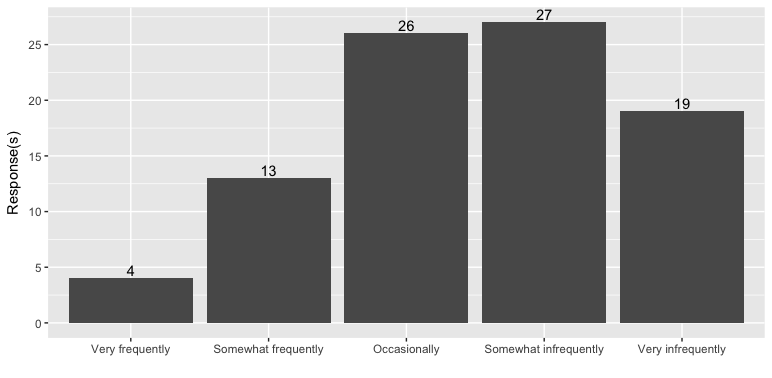
\includegraphics[width=0.95\textwidth,keepaspectratio]{FirstAttemptFailure}}
	\caption{Frequency of Failures in First Attempts at Merge Conflict Resolution. Scale: 1 is \textit{Very frequently} and 5 is \textit{very infrequently}. 89 out of 102 participants (87.26\%) indicated a frequency in the \textit{Processes Survey}~(S1).\vspace*{-0.3\baselineskip}}
	\label{fig:first-attempt-failure}
\end{figure}

Furthermore, we asked survey participants to describe their backup strategies when their first attempt at resolving a merge conflict fails.
We received 75 responses and the aggregate results are presented in Table~\ref{backup-strategies}, ranked according to the percentage of participants that described using each backup strategy.

Developers' backup strategies include \textit{take it offline} (B1), \textit{collaborating} (B2), \textit{try again} (B3), \textit{redoing changes} (B4), and \textit{no backup strategy} (B5).
Since \textit{no backup strategy} (B5) is not a strategy in and of itself, we focus on strategies B1--B4 instead.

The \textit{take it offline} (B1) strategy involves moving conflicting code away from shared branches or code repositories, and working locally to resolve the conflict without disrupting other developers.
The antithesis of this strategy is \textit{collaborating} (S2), where developers seek out other developers that are more knowledgeable about the area of conflicting code.
The B1 and B2 strategies contrast each other, and show that developers reserve more costly strategies (in terms of time, effort, and coordination) as backups to their primary resolution strategies.
The most common backup strategies, are in a way, opposite of the primary strategies.

Additionally, we find that developers also simply \textit{try again} (B3) to merge the same code together and hope that their tools are able to succeed with a second attempt.
Developers also resort to \textit{redoing changes} (B4), by way of reverting and manually recreating the changes found in conflicting commits when their initial attempt failed.
The B3 and B4 strategies appear to cement the extremes of the cost spectrum of backup strategies for resolving merge conflicts.
Simply retrying the same merge (B3) requires very little additional work.
It implies that developers think that they might have missed something, and that by going through the changes again, they might catch or have a better understanding of the two changes that are conflicting.
However, the process of redoing changes (B4) is a duplication of previous efforts. %and is therefore costly on developer's time.
This \textit{Nuclear Option} is clearly a time-consuming strategy for developers (both in planning and implementing a resolution), and yet the perceived costs of trying to unravel the conflicting code appear to be higher than the costs of reimplementing features.

\begin{table}[!htbp]
\renewcommand{\arraystretch}{1.2}
\caption{Backup Strategies for Resolving Merge Conflicts from Processes Survey (S1)}
\label{backup-strategies}
\centering
\begin{tabularx}{\textwidth}{c|l|c|r}
\toprule
  \parnoteclear % tabularx will otherwise add each note thrice
  Strategy & Description & \# Participants\parnote{75 out of 102 participants (73.53\%) provided a description of their backup strategy.\vspace*{-0.3\baselineskip}} & Percentage (\%)\textsuperscript{i} \\
\midrule
  B1 & Take it offline & 19 & 25.33\% \\
  B2 & Collaborating & 17 & 22.67\% \\
  B3 & Try again & 15 & 20.00\% \\
  B4 & Redoing changes & 14 & 18.67\% \\
  B5 & No backup strategy\hspace{2.0cm} & 10 & 13.33\% \\
\bottomrule
\end{tabularx}
\parnotes
\end{table}
\vspace{0.8em}

\boldif{Some developers do not have an approach for dealing with merge conflicts.}
Finally, an interesting result is that some developers do not have a strategy for approaching a merge conflict resolution.
The existence of this \textit{no strategy} approach is anecdotal, but curious, since we assume that developers are rational actors seeking to organize themselves in ways that increase the likelihood of successful outcomes.
Yet this strategy appears to go counter to that notion.
One explanation for the lack of a strategy is the lack of experience.
With a mean of 3.5 years of programming experience (5.6 years less than the overall mean), these participants might not have encountered enough situations to form a coherent strategy.

Interestingly, when developers perceive a merge conflict to be too difficult to resolve they occasionally resort to removing all conflicting code and reimplementing the underlying functionality in order to fix it.
